%! Author = crist
%! Date = 03/12/2025

\spacing{1.3}


\section{Energía}
\begin{definition}[Energía]
    Se define como la capacidad de un cuerpo para producir cambios en sí mismo o en su entorno
\end{definition}
La unidad de energía en el Sistema Internacional es el Julio (\unit{\joule}). Otras formas de energía y su equivalencia en julios son:
\begin{itemize}
    \item \textbf{Caloría (\unit{\calorie})}. \( \qty{1}{\calorie} = \qty{4.18}{\joule} \).
    \item \textbf{Kilovatio-hora} (\unit{\kwh}) \( \longrightarrow \) \( \qty{1}{\kwh} = \qty{3.6e6}{\joule} \)
\end{itemize}
Tenemos varias formas de energía que se pueden clasificar principalmente en:
\begin{enumerate}[label=\letraminuscula]
        \item \textbf{Energía cinética}.
        Es la energía debida al movimiento de los objetos.
        \item \textbf{Energía potencial}.
        Es la energía debida al cambio de altura de los objetos.
        \item \textbf{Energía mecánica}.
        Es la suma de la energía cinética y la energía potencial.
        \item \textbf{Energía térmica}.
        Es la energía debida al intercambio de calor (más adelante veremos la definición de calor).
        \item \textbf{Energía eólica}.
        Es la energía debida al viento.
        \item \textbf{Energía nuclear}.
        Es la energía debida al proceso de fusión o fisión nuclear.
        \item \textbf{Energía eléctrica}.
        Es la energía debida al movimiento de los electrones.
\end{enumerate}


\section{Trabajo}
\begin{definition}[Trabajo]
    Se define como la transformación producida por una fuerza, es decir, hablamos de trabajo cuando una fuerza transmite energía
\end{definition}
\begin{remark}
    La energía y el trabajo están relacionados.
\end{remark}
El trabajo mecánico se representa mediante \( W \) y su expresión es:
\vspace*{10pt}
\begin{centeredequation}
    \eqnmarkbox[red]{trabajo}{W}
    =
    \eqnmarkbox[blue]{fuerza}{F}
    \cdot
    \eqnmarkbox[mygreen]{distancia}{d}
    \label{eq:trabajo_1}
\end{centeredequation}
\annotate[yshift=1em]{left}{trabajo}{Trabajo}
\annotate[yshift=1em]{}{fuerza}{Fuerza aplicada}
\annotate[yshift=-1em]{below,left}{distancia}{Desplazamiento del objeto}
\vspace{12pt}

Esta distancia \( d \) puede representarse como la distancia final menos la distancia inicial según la expresión: \( d = x_f - x_i \)
\begin{figure}[H]
    \centering
%    \includegraphics[scale=0.75]{images/energia/trabajo_imagen}
    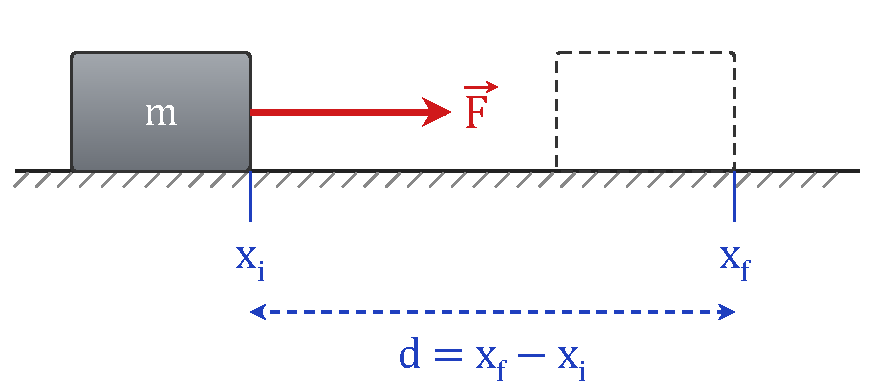
\includegraphics[width=0.7\textwidth]{Figuras_SVG_ES/pdf/U4_trabajo_desplazamiento.pdf}
    \caption{Representación del trabajo}
    \label{fig:trabajo}
\end{figure}
Cuando varias fuerzas actúan sobre el mismo cuerpo, el trabajo realizado por esas fuerzas es el mismo que el trabajo realizado por su resultante (la suma de todas ellas), es decir:
\begin{centeredequation}
    \Sigma F = F_1 + F_2 + \dots
\end{centeredequation}
Por lo tanto, la expresión anterior se convierte en:
\begin{centeredequation}
    W = \Sigma F \cdot d
    \label{eq:trabajo_2}
\end{centeredequation}
\begin{remark}
    El trabajo es una forma de energía y, por tanto, su unidad en el SI es el julio.
\end{remark}

\begin{exercise}
    Calcula el trabajo realizado por un burro cuando ejerce una fuerza de 2000 N sobre un carro y lo arrastra durante 400 metros.
    \begin{solu}
        El trabajo se calcula mediante la fórmula:
        \[
            W = F \cdot d
        \]
        Donde:
        \begin{itemize}
            \item $F = \qty{2000}{\newton}$ (fuerza aplicada)
            \item $d = \qty{400}{\metre}$ (desplazamiento)
        \end{itemize}
        Sustituyendo los valores:
        \[
            W = 2000 \times 400 = \qty{800000}{\joule} = \qty{800}{\kilo\joule}
        \]
        \textbf{Respuesta:} El burro realiza \qty{800}{\kilo\joule} de trabajo.
    \end{solu}
\end{exercise}

\begin{exercise}
    Un estudiante empuja una caja con una fuerza de 80 N y la mueve \qty{5}{\metre} en la misma dirección que la fuerza. Calcula el trabajo realizado.
    \begin{solu}
        Usando la fórmula del trabajo:
        \[
            W = F \cdot d = 80 \times 5 = \qty{400}{\joule}
        \]
        \textbf{Respuesta:} El trabajo realizado es \qty{400}{\joule}.
    \end{solu}
\end{exercise}

\begin{exercise}
    Un coche es empujado por cuatro personas que ejercen una fuerza total de \qty{600}{\newton}. Si el coche se mueve 8 metros, ¿qué trabajo han realizado?
    \begin{solu}

        \[
            W = F \cdot d = 600 \times 8 = \qty{4800}{\joule} = \qty{4.8}{\kilo\joule}
        \]
        \textbf{Respuesta:} Han realizado \qty{4.8}{\kilo\joule} de trabajo.
    \end{solu}
\end{exercise}

\begin{exercise}
    Una persona arrastra una maleta por el suelo aplicando una fuerza de \qty{45}{\newton} en un desplazamiento de \qty{25}{\metre}. Calcula el trabajo realizado.
    \begin{solu}
        \[
            W = F \cdot d = 45 \times 25 = \qty{1125}{\joule} = \qty{1.125}{\kilo\joule}
        \]
        \textbf{Respuesta:} El trabajo realizado es \qty{1.125}{\kilo\joule}.
    \end{solu}
\end{exercise}

\begin{exercise}
    Encuentra el trabajo neto necesario para mover un bloque de \qty{10}{\kilo\gram} cuando el cuerpo se desplaza 3 metros, con fuerzas $F_1 = \qty{80}{\newton}$ y $F_2 = \qty{15}{\newton}$ actuando en la misma dirección.
    \begin{solu}
        Primero, calculamos la fuerza neta:
        \[
            F_{net} = F_1 + F_2 = 80 + 15 = \qty{95}{\newton}
        \]
        Después, calculamos el trabajo:
        \[
            W = F_{net} \cdot d = 95 \times 3 = \qty{285}{\joule}
        \]
        \textbf{Respuesta:} El trabajo neto es \qty{285}{\joule}.
    \end{solu}
\end{exercise}

\begin{exercise}
    Un albañil utiliza una polea para levantar una masa de 50 kg hasta una altura de 10 m. ¿Qué trabajo se ha realizado? (Datos: $g = \qty{9.8}{\mpss}$)
    \begin{solu}
        Primero, calculamos el peso (fuerza):
        \[
            F = m \cdot g = 50 \times 9.8 = \qty{490}{\newton}
        \]
        Después, calculamos el trabajo:
        \[
            W = F \cdot h = 490 \times 10 = \qty{4900}{\joule} = \qty{4.9}{\kilo\joule}
        \]
        \textbf{Respuesta:} El trabajo realizado es \qty{4.9}{\kilo\joule}.
    \end{solu}
\end{exercise}


\section{Energía cinética}

La energía cinética es la energía que posee un cuerpo cuando está en movimiento.
La expresión matemática de la energía cinética es:

\vspace{12pt}
\begin{centeredequation}
    \eqnmarkbox[red]{energiacinetica}{E_k}
    =
    \dfrac{1}{2}
    \eqnmarkbox[blue]{masa}{m}
    \cdot
    \eqnmarkbox[mygreen]{velocidad}{v^2}
    \label{eq:energia_cinetica}
\end{centeredequation}
\annotate[yshift=1em]{left}{energiacinetica}{Energía cinética}
\annotate[yshift=1em]{}{masa}{masa}
\annotate[yshift=-1em]{below,left}{velocidad}{velocidad}
\vspace{12pt}


\begin{exercise}
    Un coche de 1000 kg viaja a una velocidad de 20 m/s. Calcula su energía cinética.
    \begin{solu}
        La fórmula de la energía cinética es:
        \[
            E_k = \frac{1}{2}mv^2
        \]
        Donde $m = \qty{1000}{\kilo\gram}$ y $v = \qty{20}{\mps}$:
        \[
            E_k = \frac{1}{2} \times 1000 \times 20^2 = \frac{1}{2} \times 1000 \times 400 = \qty{200000}{\joule} = \qty{200}{\kilo\joule}
        \]
        \textbf{Respuesta:} La energía cinética es \qty{200}{\kilo\joule}.
    \end{solu}
\end{exercise}

\begin{exercise}
    Una pelota de 0,5 kg se mueve con una velocidad de 10 m/s. ¿Cuál es su energía cinética?
    \begin{solu}
        \[
            E_k = \frac{1}{2}mv^2 = \frac{1}{2} \times 0.5 \times 10^2 = 0.25 \times 100 = \qty{25}{\joule}
        \]
        \textbf{Respuesta:} La energía cinética es \qty{25}{\joule}.
    \end{solu}
\end{exercise}

\begin{exercise}
    Si un objeto de 4 kg tiene una energía cinética de 200 J, ¿a qué velocidad se mueve?
    \begin{solu}
        A partir de $E_k = \frac{1}{2}mv^2$, despejamos $v$:
        \[
            v = \sqrt{\frac{2E_k}{m}} = \sqrt{\frac{2 \times 200}{4}} = \sqrt{\frac{400}{4}} = \sqrt{100} = \qty{10}{\mps}
        \]
        \textbf{Respuesta:} El objeto se mueve a \qty{10}{\mps}.
    \end{solu}
\end{exercise}

\begin{exercise}
    ¿Cuál es la velocidad de un atleta de 80 kg que tiene una energía cinética de 8000 J?
    \begin{solu}
        \[
            v = \sqrt{\frac{2E_k}{m}} = \sqrt{\frac{2 \times 8000}{80}} = \sqrt{\frac{16000}{80}} = \sqrt{200} \approx \qty{14.14}{\mps}
        \]
        \textbf{Respuesta:} El atleta se mueve a aproximadamente \qty{14.14}{\mps}.
    \end{solu}
\end{exercise}


\section{Energía potencial}

Tenemos dos tipos de energía potencial: la energía potencial gravitatoria y la energía potencial elástica.

\subsection{Energía potencial gravitatoria}

Esta energía es consecuencia de la posición de un cuerpo (altura).
La expresión matemática de la energía potencial es:

\vspace{6pt}
\begin{centeredequation}
    \eqnmarkbox[red]{energiapotencial}{E_p}
    =
    \eqnmarkbox[blue]{masa}{m}
    \cdot
    \eqnmarkbox[mygreen]{gravedad}{g}
    \cdot
    \eqnmarkbox[myOrange]{altura}{h}
    \label{eq:energia_potencial}
\end{centeredequation}
\annotate[yshift=1em]{left}{energiapotencial}{Energía potencial}
\annotate[yshift=1em]{}{masa}{masa}
\annotate[yshift=-1em]{below,left}{gravedad}{gravedad}
\annotate[yshift=-1em]{below,right}{altura}{altura}
\vspace{12pt}


\begin{remark}
    A la energía potencial gravitatoria se la conoce habitualmente simplemente como energía potencial.
\end{remark}



\begin{exercise}
    Un libro de 2 kg está en una estantería a 1,5 m de altura. Calcula su energía potencial gravitatoria. (Datos: $g = 9.8$ m/s$^2$)
    \begin{solu}
        La fórmula de la energía potencial gravitatoria es:
        \[
            E_p = mgh
        \]
        Donde $m = \qty{2}{\kilo\gram}$, $g = \qty{9.8}{\mpss}$, y $h = \qty{1.5}{\metre}$:
        \[
            E_p = 2 \times 9.8 \times 1.5 = \qty{29.4}{\joule}
        \]
        \textbf{Respuesta:} La energía potencial es \qty{29.4}{\joule}.
    \end{solu}
\end{exercise}

\begin{exercise}
    Una maceta de 5 kg está situada en un balcón a 12 m del suelo. ¿Cuál es su energía potencial gravitatoria?
    \begin{solu}
        \[
            E_p = mgh = 5 \times 9.8 \times 12 = \qty{588}{\joule}
        \]
        \textbf{Respuesta:} La energía potencial es \qty{588}{\joule}.
    \end{solu}
\end{exercise}

\begin{exercise}
    Si un objeto tiene una energía potencial de 600 J y está situado a 3 m de altura, ¿cuál es su masa?
    \begin{solu}
        A partir de $E_p = mgh$, despejamos $m$:
        \[
            m = \frac{E_p}{gh} = \frac{600}{9.8 \times 3} = \frac{600}{29.4} \approx \qty{20.41}{\kilo\gram}
        \]
        \textbf{Respuesta:} La masa es aproximadamente \qty{20.41}{\kilo\gram}.
    \end{solu}
\end{exercise}

\begin{exercise}
    ¿A qué altura debe elevarse un objeto de 2 kilogramos para que su energía potencial sea de 125 J?
    \begin{solu}
        A partir de $E_p = mgh$, despejamos $h$:
        \[
            h = \frac{E_p}{mg} = \frac{125}{2 \times 9.8} = \frac{125}{19.6} \approx \qty{6.38}{\metre}
        \]
        \textbf{Respuesta:} El objeto debe elevarse a aproximadamente \qty{6.38}{\metre}.
    \end{solu}
\end{exercise}


\section{Energía mecánica}

La energía mecánica es la suma de la energía cinética y la energía potencial.

\begin{centeredequation}
    E_m = E_k + E_p
    \label{eq:energia_mecanica}
\end{centeredequation}

\begin{exercise}
    Calcula la energía de los siguientes objetos:
    \begin{enumerate}[label=\alph*)]
\item Un coche de 1200 kg que viaja a una velocidad de \qty{6}{\mps}
\item Un marco de fotos de 450 gramos situado a 1,75 metros del suelo.
\item Una pelota de tenis de 60 gramos con una velocidad de \qty{65}{\mps} y una altura de 1,25 metros.
    \end{enumerate}
    \begin{solu}
        a) Solo energía cinética:
        \[
            E_k = \frac{1}{2} \times 1200 \times 6^2 = \frac{1}{2} \times 1200 \times 36 = \qty{21600}{\joule} = \qty{21.6}{\kilo\joule}
        \]
        b) Solo energía potencial (convertimos a kg: 450 g = 0,45 kg):
        \[
            E_p = 0.45 \times 9.8 \times 1.75 = \qty{7.72}{\joule}
        \]
        c) Energía cinética y potencial (convertimos a kg: 60 g = 0,06 kg):
        \[
            E_k = \frac{1}{2} \times 0.06 \times 65^2 = \frac{1}{2} \times 0.06 \times 4225 = \qty{126.75}{\joule}
        \]
        \[
            E_p = 0.06 \times 9.8 \times 1.25 = \qty{0.735}{\joule}
        \]
        \[
            E_M = E_k + E_p = 126.75 + 0.735 = \qty{127.49}{\joule}
        \]
        \textbf{Respuestas:} a) \qty{21.6}{\kilo\joule}, b) \qty{7.72}{\joule}, c) \qty{127.49}{\joule}
    \end{solu}
\end{exercise}

\begin{exercise}
    Encuentra la energía mecánica de un águila de 2500 gramos que vuela a una velocidad de \qty{100}{\kmph} y a una altura de 250 m.
    \begin{solu}
        Primero, convertimos las unidades:
        \begin{itemize}
            \item Masa: 2500 g = 2,5 kg
            \item Velocidad: 100 km/h = $\frac{100 \times 1000}{3600} = \qty{27.78}{\mps}$
        \end{itemize}
        Calculamos la energía cinética:
        \[
            E_k = \frac{1}{2} \times 2.5 \times 27.78^2 = \frac{1}{2} \times 2.5 \times 771.73 = \qty{964.66}{\joule}
        \]

        Calculamos la energía potencial:
        \[
            E_p = 2.5 \times 9.8 \times 250 = \qty{6125}{\joule}
        \]

        Energía mecánica total:
        \[
            E_M = E_k + E_p = 964.66 + 6125 = \qty{7089.66}{\joule} \approx \qty{7.09}{\kilo\joule}
        \]
        \textbf{Respuesta:} La energía mecánica es aproximadamente \qty{7.09}{\kilo\joule}.
    \end{solu}
\end{exercise}

\begin{exercise}
    De las siguientes situaciones, ¿cuál tendrá la mayor energía mecánica?:
    \begin{enumerate}[label=\alph*)]
\item Una roca de 10 kg a una altura de 5 metros.
\item Una roca de 5 kg a una altura de 10 metros.
\item Un dron de 250 gramos que vuela cerca del suelo a una velocidad de \qty{25}{\mps}
\item Una piedra de 500 gramos a una altura de 250 metros y una velocidad de \qty{10}{\mps}
    \end{enumerate}
    \begin{solu}
        a) $E_p = 10 \times 9.8 \times 5 = \qty{490}{\joule}$

        b) $E_p = 5 \times 9.8 \times 10 = \qty{490}{\joule}$

        c) $E_k = \frac{1}{2} \times 0.25 \times 25^2 = \frac{1}{2} \times 0.25 \times 625 = \qty{78.13}{\joule}$

        d) $E_k = \frac{1}{2} \times 0.5 \times 10^2 = 25$ J; $E_p = 0.5 \times 9.8 \times 250 = 1225$ J; $E_M = \qty{1250}{\joule}$

        \textbf{Respuesta:} La opción d) tiene la mayor energía mecánica con \qty{1250}{\joule}.
    \end{solu}
\end{exercise}

\begin{exercise}
    Una pelota de 0,4 kg está a una altura de 5 m y se mueve con una velocidad de 8 m/s. Calcula:
    \begin{enumerate}
        \item Su energía potencial
        \item Su energía cinética
        \item Su energía mecánica total
    \end{enumerate}
    \begin{solu}
        1. Energía potencial:
        \[
            E_p = 0.4 \times 9.8 \times 5 = \qty{19.6}{\joule}
        \]
        2. Energía cinética:
        \[
            E_k = \frac{1}{2} \times 0.4 \times 8^2 = 0.2 \times 64 = \qty{12.8}{\joule}
        \]
        3. Energía mecánica total:
        \[
            E_M = E_p + E_k = 19.6 + 12.8 = \qty{32.4}{\joule}
        \]
        \textbf{Respuestas:} 1) \qty{19.6}{\joule}, 2) \qty{12.8}{\joule}, 3) \qty{32.4}{\joule}
    \end{solu}
\end{exercise}

\begin{exercise}
    Un pájaro de 0,2 kg vuela a una altura de 15 m con una velocidad de 12 m/s. Determina su energía mecánica total.
    \begin{solu}
        Energía cinética:
        \[
            E_k = \frac{1}{2} \times 0.2 \times 12^2 = 0.1 \times 144 = \qty{14.4}{\joule}
        \]
        Energía potencial:
        \[
            E_p = 0.2 \times 9.8 \times 15 = \qty{29.4}{\joule}
        \]
        Energía mecánica total:
        \[
            E_M = 14.4 + 29.4 = \qty{43.8}{\joule}
        \]
        \textbf{Respuesta:} La energía mecánica total es \qty{43.8}{\joule}.
    \end{solu}
\end{exercise}


\section{Principio de conservación de la energía mecánica}


\begin{dBox}
    \textbf{El principio de conservación de la energía mecánica dice}: la energía mecánica al principio (fijamos un punto inicial, representado en la fórmula con \( i \)) será igual a la energía mecánica al final (fijamos el punto final, representado en la fórmula con \( f \))
\end{dBox}

Matemáticamente, este principio se puede expresar como:
\begin{centeredequation}
    E_{m,i} = E_{m,f}
    \label{eq:conservacion_energia}
\end{centeredequation}
Esta expresión también se puede escribir como:
\begin{centeredequation}
    E_{p,i} + E_{c,i}  = E_{p,f} + E_{c,f}
    \label{eq:conservacion_energia_semidesarrollada}
\end{centeredequation}
Si desarrollamos aún más esta expresión, obtenemos:
\begin{centeredequation}
    m\cdot g \cdot h_i + \dfrac{1}{2} \cdot m\ v_i^2 = m\cdot g \cdot h_f + \dfrac{1}{2} \cdot m\ v_f^2
    \label{eq:conservacion_energia_desarrollada}
\end{centeredequation}

\begin{exercise}
    Una esfera metálica de 50 kg se deja caer desde una altura de 8 metros hasta el suelo.
    \begin{enumerate}[label=\alph*)]
\item Calcula la energía mecánica que tiene en el momento en que se deja caer.
\item ¿Con qué velocidad llega al suelo?
    \end{enumerate}
    \begin{solu}
        a) En el momento de la suelta, toda la energía es potencial:
        \[
            E_M = E_p = mgh = 50 \times 9.8 \times 8 = \qty{3920}{\joule}
        \]
        b) Por conservación de la energía, a nivel del suelo toda la energía es cinética:
        \[
            E_k = E_M \Rightarrow \frac{1}{2}mv^2 = 3920
        \]
        \[
            v = \sqrt{\frac{2 \times 3920}{50}} = \sqrt{\frac{7840}{50}} = \sqrt{156.8} \approx \qty{12.52}{\mps}
        \]
        Alternativamente: $v = \sqrt{2gh} = \sqrt{2 \times 9.8 \times 8} = \sqrt{156.8} \approx \qty{12.52}{\mps}$
        \textbf{Respuestas:} a) \qty{3920}{\joule}, b) \qty{12.52}{\mps}
    \end{solu}
\end{exercise}

\begin{exercise}
    Desde una altura de \qty{15}{\metre}, un objeto de masa \qty{3}{\kilo\gram} se lanza verticalmente hacia abajo con una velocidad inicial de \qty{2}{\mps}. Si no hay resistencia del aire, encuentra:
    \begin{enumerate}[label=\alph*)]
\item La energía cinética a 5 metros sobre el suelo.
\item La velocidad en ese momento y la velocidad con la que llega al suelo.
    \end{enumerate}
    \begin{solu}
        Energía inicial (a h = 15 m):
        \[
            E_k = \frac{1}{2} \times 3 \times 2^2 = \qty{6}{\joule}
        \]
        \[
            E_p = 3 \times 9.8 \times 15 = \qty{441}{\joule}
        \]
        \[
            E_{M,initial} = 6 + 441 = \qty{447}{\joule}
        \]
        a) A h = 5 m:
        \[
            E_p = 3 \times 9.8 \times 5 = \qty{147}{\joule}
        \]
        \[
            E_k = E_M - E_p = 447 - 147 = \qty{300}{\joule}
        \]
        b) Velocidad a h = 5 m:
        \[
            v = \sqrt{\frac{2E_k}{m}} = \sqrt{\frac{2 \times 300}{3}} = \sqrt{200} \approx \qty{14.14}{\mps}
        \]
        Velocidad en el suelo (h = 0):
        \[
            E_k = E_M = 447 \text{ J}
        \]
        \[
            v = \sqrt{\frac{2 \times 447}{3}} = \sqrt{298} \approx \qty{17.26}{\mps}
        \]
        \textbf{Respuestas:} a) \qty{300}{\joule}, b) \qty{14.14}{\mps} a 5 m de altura, \qty{17.26}{\mps} en el suelo
    \end{solu}
\end{exercise}

\begin{exercise}
    En un tobogán de 2 metros de altura hay un niño de 25 kg. ¿Con qué velocidad llegaría al suelo al deslizarse?
    \begin{solu}
        Por conservación de la energía:
        \[
            E_{p,initial} = E_{k,final}
        \]
        \[
            mgh = \frac{1}{2}mv^2
        \]
        \[
            v = \sqrt{2gh} = \sqrt{2 \times 9.8 \times 2} = \sqrt{39.2} \approx \qty{6.26}{\mps}
        \]
        \textbf{Respuesta:} El niño llega al suelo a aproximadamente \qty{6.26}{\mps}.
    \end{solu}
\end{exercise}

\begin{exercise}
    Una pelota de 0,5 kg se deja caer desde una ventana a 30 m sobre la calle. Calcula:
    \begin{enumerate}[label=\alph*)]
\item La energía potencial respecto al suelo en el momento de la suelta.
\item La energía cinética en el momento en que llega al suelo.
\item La velocidad con la que golpea el suelo.
    \end{enumerate}
    \begin{solu}
        a) Energía potencial en el momento de la suelta:
        \[
            E_p = 0.5 \times 9.8 \times 30 = \qty{147}{\joule}
        \]
        b) Por conservación de la energía, toda la energía potencial se convierte en cinética:
        \[
            E_k = \qty{147}{\joule}
        \]
        c) Velocidad en el suelo:
        \[
            v = \sqrt{2gh} = \sqrt{2 \times 9.8 \times 30} = \sqrt{588} \approx \qty{24.25}{\mps}
        \]
        \textbf{Respuestas:} a) \qty{147}{\joule}, b) \qty{147}{\joule}, c) \qty{24.25}{\mps}
    \end{solu}
\end{exercise}

\begin{exercise}
    En lo alto de una montaña rusa, un vagón y sus ocupantes con una masa total de 1000 kg están a una altura de 50 metros sobre el suelo y tienen una velocidad de \qty{5}{\mps}.
    \begin{enumerate}[label=\alph*)]
\item ¿Qué velocidad tendrá el vagón cuando llegue a la siguiente cima, que está a una altura de 25 metros sobre el suelo?
\item Si la velocidad que tiene en la siguiente cima es de \qty{20}{\mps}, ¿cuál es el trabajo realizado por el rozamiento entre las ruedas y los raíles?
    \end{enumerate}
    \begin{solu}
        Energía inicial (\( h_1 = \qty{50}{\metre} \), \( v_1 = \qty{5}{\metre\per\second} \)):
        \[
            E_{M1} = \frac{1}{2} \times 1000 \times 5^2 + 1000 \times 9.8 \times 50 = 12500 + 490000 = \qty{502500}{\joule}
        \]
        a) Sin rozamiento, a \( h_2 = \qty{25}{\metre} \):
        \[
            E_p = 1000 \times 9.8 \times 25 = \qty{245000}{\joule}
        \]
        \[
            E_k = E_{M1} - E_p = 502500 - 245000 = \qty{257500}{\joule}
        \]
        \[
            v = \sqrt{\frac{2 \times 257500}{1000}} = \sqrt{515} \approx \qty{22.69}{\mps}
        \]
        b) Energía real en \( h_2 \) con \( v_2 \) = \qty{20}{\metre\per\second}:
        \[
            E_{M2} = \frac{1}{2} \times 1000 \times 20^2 + 245000 = 200000 + 245000 = \qty{445000}{\joule}
        \]
        Trabajo realizado por el rozamiento (negativo porque se opone al movimiento):
        \[
            W_{friction} = E_{M2} - E_{M1} = 445000 - 502500 = \qty{-57500}{\joule}
        \]
        \textbf{Respuestas:} a) \qty{22.69}{\mps}, b) \qty{-57500}{\joule} (o \qty{57500}{\joule} de energía perdida)
    \end{solu}
\end{exercise}

\begin{exercise}
    Una pelota de 0,3 kg se deja caer desde una altura de 10 m. Calcula:
    \begin{enumerate}
        \item La energía mecánica inicial
        \item La velocidad con la que llega al suelo
        \item La energía cinética justo antes de tocar el suelo
    \end{enumerate}
    \begin{solu}
        1. Energía mecánica inicial (toda potencial):
        \[
            E_M = mgh = 0.3 \times 9.8 \times 10 = \qty{29.4}{\joule}
        \]
        2. Velocidad en el suelo:
        \[
            v = \sqrt{2gh} = \sqrt{2 \times 9.8 \times 10} = \sqrt{196} = \qty{14}{\mps}
        \]
        3. Energía cinética en el suelo (igual a la energía mecánica inicial):
        \[
            E_k = \qty{29.4}{\joule}
        \]
        \textbf{Respuestas:} 1) \qty{29.4}{\joule}, 2) \qty{14}{\mps}, 3) \qty{29.4}{\joule}
    \end{solu}
\end{exercise}

\begin{exercise}
    Un péndulo tiene una masa de 0,5 kg y se suelta desde una altura de 2 m. Si no hay rozamiento:
    \begin{enumerate}
        \item ¿Cuál es su energía potencial inicial?
        \item ¿Cuál será su velocidad máxima en el punto más bajo?
        \item ¿Qué energía cinética tendrá cuando esté a una altura de 1 m?
    \end{enumerate}
    \begin{solu}
        1. Energía potencial inicial:
        \[
            E_p = 0.5 \times 9.8 \times 2 = \qty{9.8}{\joule}
        \]
        2. Velocidad máxima en el punto más bajo (h = 0):
        \[
            v = \sqrt{2gh} = \sqrt{2 \times 9.8 \times 2} = \sqrt{39.2} \approx \qty{6.26}{\mps}
        \]
        3. A h = 1 m:
        \[
            E_p = 0.5 \times 9.8 \times 1 = \qty{4.9}{\joule}
        \]
        \[
            E_k = E_M - E_p = 9.8 - 4.9 = \qty{4.9}{\joule}
        \]
        \textbf{Respuestas:} 1) \qty{9.8}{\joule}, 2) \qty{6.26}{\mps}, 3) \qty{4.9}{\joule}
    \end{solu}
\end{exercise}

\begin{exercise}
    Un esquiador de 70 kg parte del reposo desde la cima de una pendiente situada a 20 m de altura. Si despreciamos el rozamiento, ¿con qué velocidad llegará a la base de la pendiente?
    \begin{solu}
        Usando la conservación de la energía:
        \[
            v = \sqrt{2gh} = \sqrt{2 \times 9.8 \times 20} = \sqrt{392} \approx \qty{19.80}{\mps}
        \]
        \textbf{Respuesta:} El esquiador llegará a la base a aproximadamente \qty{19.80}{\mps}.
    \end{solu}
\end{exercise}


\section{Potencia}

Otra magnitud importante es la potencia (\( P \)). La potencia se puede definir como la energía (\( E \)) o el trabajo (\( W \)) realizado por unidad de tiempo (\( t \)), y su expresión matemática es:
\begin{centeredequation}
    P = \dfrac{E}{t}
    \label{eq:potencia_energia}
\end{centeredequation}
o de forma equivalente:
\begin{centeredequation}
    P = \dfrac{W}{t}
    \label{eq:potencia_trabajo}
\end{centeredequation}

La unidad de potencia en el Sistema Internacional es el Vatio (\unit{\watt}). Otra unidad de potencia muy utilizada es el caballo de vapor (CV), donde
\( 1\ HP = \qty{735}{\watt} \)

\begin{exercise}
    Una grúa levanta una carga de $500\,\text{kg}$ hasta una altura de $20\,\text{metros}$ en $10\,\text{segundos}$. Calcula la potencia desarrollada por la grúa. (Usa $g = 9.8\,\text{m/s}^2$).
    \begin{solu}
        Primero, calculamos el trabajo realizado (energía potencial): $W = m \cdot g \cdot h$ \\
        $W = 500\,\text{kg} \cdot 9.8\,\text{m/s}^2 \cdot 20\,\text{m} = 98,000\,\text{J}$ \\
        Ahora, hallamos la potencia: $P = \frac{W}{t} = \frac{98,000\,\text{J}}{10\,\text{s}} = \mathbf{9800\,\text{W}}$
    \end{solu}
\end{exercise}

\begin{exercise}
    Un motor eléctrico tiene una potencia de $1200\,\text{W}$. ¿Cuánto tiempo tardará en realizar $18,000\,\text{J}$ de trabajo?
    \begin{solu}
        Usando la fórmula $P = \frac{W}{t}$, despejamos $t$: \\
        $t = \frac{W}{P} = \frac{18,000\,\text{J}}{1200\,\text{W}} = \mathbf{15\,\text{segundos}}$
    \end{solu}
\end{exercise}

\begin{exercise}
    Un estudiante con una masa de $60\,\text{kg}$ sube una escalera de $5\,\text{metros}$ de altura en $12\,\text{segundos}$.
    Calcula la potencia generada.
    \begin{solu}
        $W = m \cdot g \cdot h = 60\,\text{kg} \cdot 9.8\,\text{m/s}^2 \cdot 5\,\text{m} = 2940\,\text{J}$ \\
        $P = \frac{2940\,\text{J}}{12\,\text{s}} = \mathbf{245\,\text{W}}$
    \end{solu}
\end{exercise}

\begin{exercise}
    Una bombilla tiene una potencia de $60\,\text{W}$.
    Si permanece encendida durante $2\,\text{horas}$, ¿cuánta energía total (en julios) consume?
    \begin{solu}
        Primero, convertimos el tiempo a segundos: $2\,\text{h} \cdot 3600\,\text{s/h} = 7200\,\text{s}$ \\
        $E = P \cdot t = 60\,\text{W} \cdot 7200\,\text{s} = \mathbf{432,000\,\text{J}}$ (o $4.32 \cdot 10^5\,\text{J}$)
    \end{solu}
\end{exercise}


\section{Consumo energético doméstico}

La Figura \ref{fig:factura_luz} muestra la información que se suele encontrar en una factura de la luz.

\begin{figure}[H]
    \centering
%    \includegraphics[scale=0.9]{images/energia/factura_luz}
    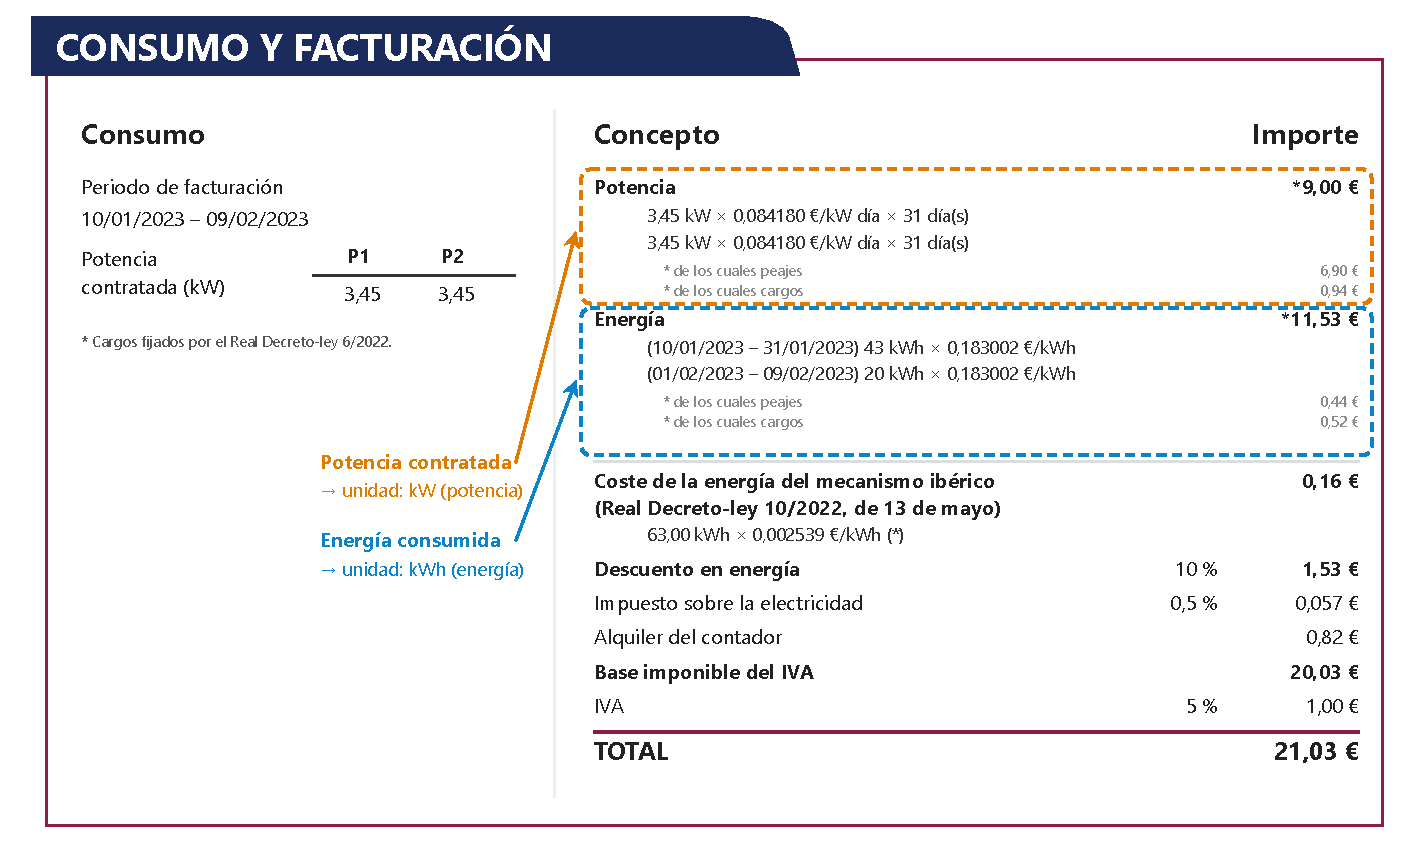
\includegraphics[width=\textwidth]{Figuras_SVG_ES/pdf/U4_factura_luz.pdf}
    \caption{Información que aparece en una factura de la luz}
    \label{fig:factura_luz}
\end{figure}

Primero, vemos que debemos pagar por la potencia contratada.
Como hemos visto, la potencia es la energía suministrada por unidad de tiempo, y su unidad en el SI es el vatio (\unit{\watt}).

En este caso, la potencia contratada es de \qty{3.45}{\kilo\watt}.
F
\begin{remark}
    Aquí vemos una conversión de unidades usando factores de conversión para calcular el precio que debemos pagar tras 31 días por la potencia contratada.
\end{remark}
\begin{example}
    Calcula el precio que tenemos que pagar por 31 días usando factores de conversión. A continuación, se muestra la energía consumida así como el precio a pagar.
    En este caso, es \( 0.084180 \dfrac{\text{€}}{\unit{\kwh}} \) y vemos que primero se consumieron \qty{43}{\kwh}, seguidos de \qty{20}{\kwh}.
\end{example}


\begin{remark}
    Es importante no confundir \unit{\kwh}, que es una unidad de energía, con \unit{\watt}, que es una unidad de potencia.\\
    Calcula la equivalencia entre \unit{\kwh} y julios.
\end{remark}

\begin{exercise}
    Debes revisar una factura de electricidad doméstica y calcular el coste de tener tres electrodomésticos encendidos durante un cierto periodo de tiempo.
\end{exercise}


\section{Fuentes de energía}

Una \textbf{fuente de energía} es un recurso natural del cual se puede obtener energía y transformarla en otras formas.
Según su capacidad de regeneración, tenemos:

\begin{enumerate}[label=\numberballmDarkTeal]
\item \negsubro{Renovables}.
La tasa de regeneración iguala a la tasa de consumo, y pueden considerarse inagotables.
\begin{itemize}
    \item Energía hidroeléctrica.
    \item Energía solar.
    \item Energía geotérmica.
    \item Biomasa.
    \item Energía marina.
    \item Energía eólica.
\end{itemize}
\item \negsubro{No renovables}
\end{enumerate}


\section{Calor y temperatura}

A menudo se confunden los términos calor y temperatura.

\textbf{Calor} es la cantidad de energía transferida de un cuerpo a otro debido a una diferencia de temperatura.
Para que exista calor, dos cuerpos deben estar en contacto.
Dado que el calor es una forma de energía, su unidad en el SI es el julio.

\textbf{Temperatura} es la medida de la energía cinética de las moléculas de una sustancia.
La unidad del SI es el Kelvin, aunque los grados Celsius se usan ampliamente.

\begin{centeredequation}
    \unit{\kelvin} = \unit{\degreeCelsius} + 273
\end{centeredequation}
\begin{centeredequation}
    \unit{\degreeCelsius} = \unit{\kelvin} - 273
\end{centeredequation}

\begin{remark}
    Podemos decir que la temperatura es muy alta pero el calor es bajo.\\
    ¿Podrías explicar por qué?
\end{remark}

\begin{exercise}
    Explica por qué la temperatura en la superficie del sol es muy alta, mientras que su calor no es tan alto en comparación.
    Busca la respuesta en internet, incluyendo fuentes relevantes.
\end{exercise}

%\section{Vocabulario}
%
%
%\begin{vocabulary}[Energy]
%The capacity to do work or produce change in a physical system. \newline
%\textbf{Translation to Spanish}: Energía \newline
%% Line 10
%\end{vocabulary}
%
%
%\begin{vocabulary}[Kinetic Energy]
%The energy possessed by an object due to its motion. \newline
%\textbf{Translation to Spanish}: Energía cinética \newline
%% Line 52
%\end{vocabulary}
%
%
%\begin{vocabulary}[Potential Energy]
%Stored energy associated with the position or configuration of an object. \newline
%\textbf{Translation to Spanish}: Energía potencial \newline
%% Line 73
%\end{vocabulary}
%
%
%\begin{vocabulary}[Mechanical Energy]
%The sum of kinetic and potential energy in a system. \newline
%\textbf{Translation to Spanish}: Energía mecánica \newline
%% Line 89
%\end{vocabulary}
%
%
%\begin{vocabulary}[Work]
%The transfer of energy that occurs when a force moves an object through a distance. \newline
%\textbf{Translation to Spanish}: Trabajo \newline
%% Line 132
%\end{vocabulary}
%
%
%\begin{vocabulary}[Power]
%The rate at which work is done or energy is transferred. \newline
%\textbf{Translation to Spanish}: Potencia \newline
%% Line 174
%\end{vocabulary}
%
%
%\begin{vocabulary}[Conservation of Energy]
%A principle stating that energy cannot be created or destroyed, only transformed from one form to another. \newline
%\textbf{Translation to Spanish}: Conservación de la energía \newline
%% Line 214
%\end{vocabulary}
%
%
%\begin{vocabulary}[Thermal Energy]
%The internal energy of a system associated with the random motion of its particles. \newline
%\textbf{Translation to Spanish}: Energía térmica \newline
%% Line 247
%\end{vocabulary}
%
%
%\begin{vocabulary}[Heat]
%The transfer of thermal energy between systems due to a temperature difference. \newline
%\textbf{Translation to Spanish}: Calor \newline
%% Line 281
%\end{vocabulary}
%
%
%\begin{vocabulary}[Temperature]
%A measure of the average kinetic energy of the particles in a substance. \newline
%\textbf{Translation to Spanish}: Temperatura \newline
%% Line 298
%\end{vocabulary}
